%----------------------------------------------------------------------------------------
%	PACKAGES AND OTHER DOCUMENT CONFIGURATIONS
%----------------------------------------------------------------------------------------

\documentclass{article}

\usepackage{fancyhdr} % Required for custom headers
\usepackage{lastpage} % Required to determine the last page for the footer
\usepackage{extramarks} % Required for headers and footers
\usepackage[usenames,dvipsnames]{color} % Required for custom colors
\usepackage{graphicx} % Required to insert images
\usepackage{listings} % Required for insertion of code
\usepackage{courier} % Required for the courier font
\usepackage{lipsum} % Used for inserting dummy 'Lorem ipsum' text into the template
\usepackage{amsmath,xparse}
%\usepackage{minted}
\usepackage{SASnRdisplay}
\usepackage{minted}
\newminted{python}{frame=lines,framerule=2pt}
% Margins
\topmargin=-0.45in
\evensidemargin=0in
\oddsidemargin=0in
\textwidth=6.5in
\textheight=9.0in
\headsep=0.25in

\linespread{1.1} % Line spacing

% Set up the header and footer
\pagestyle{fancy}
\lhead{\hmwkAuthorName} % Top left header
\chead{\hmwkTitle} % Top center head
%\rhead{\firstxmark} % Top right header
\lfoot{\lastxmark} % Bottom left footer
\cfoot{} % Bottom center footer
\rfoot{Page\ \thepage\ of\ \protect\pageref{LastPage}} % Bottom right footer
\renewcommand\headrulewidth{0.4pt} % Size of the header rule
\renewcommand\footrulewidth{0.4pt} % Size of the footer rule

\setlength\parindent{0pt} % Removes all indentation from paragraphs

\newsavebox{\fminipagebox}
\NewDocumentEnvironment{fminipage}{m O{\fboxsep}}
{\par\kern#2\noindent\begin{lrbox}{\fminipagebox}
		\begin{minipage}{#1}\ignorespaces}
		{\end{minipage}\end{lrbox}%
	\makebox[#1]{%
		\kern\dimexpr-\fboxsep-\fboxrule\relax
		\fbox{\usebox{\fminipagebox}}%
		\kern\dimexpr-\fboxsep-\fboxrule\relax
	}\par\kern#2
}

\graphicspath{{./figs/}}

\usepackage{xcolor}
%\usepackage{listings}
\lstset{% 
	basicstyle=\small\ttfamily\bfseries,
	columns=flexible,
	language=SAS,
	keywordstyle=\color{blue}\bfseries,
	commentstyle=\color{green},
	morecomment=[f]{*},
	morecomment=[s]{/*}{*/},
	morecomment=[n]{/*}{*/},  
	escapechar=|,
	otherkeywords={!,!=,~,$,\&,_,<,>=,=<,>},
	stringstyle=\color[rgb]{0.639,0.082,0.082}\ttfamily,
	showstringspaces=false,
	keepspaces=true,
	sensitive=false,
}

\newenvironment{saslst}{\VerbatimEnvironment\noindent\begin{minipage}{\linewidth}\begin{lstlisting}}
{\end{lstlisting}\end{minipage}}

%----------------------------------------------------------------------------------------
%	DOCUMENT STRUCTURE COMMANDS
%	Skip this unless you know what you're doing
%----------------------------------------------------------------------------------------

% Header and footer for when a page split occurs within a problem environment
\newcommand{\enterProblemHeader}[1]{
\nobreak\extramarks{#1}{#1 continued on next page\ldots}\nobreak
\nobreak\extramarks{#1 (continued)}{#1 continued on next page\ldots}\nobreak
}

% Header and footer for when a page split occurs between problem environments
\newcommand{\exitProblemHeader}[1]{
\nobreak\extramarks{#1 (continued)}{#1 continued on next page\ldots}\nobreak
\nobreak\extramarks{#1}{}\nobreak
}

\setcounter{secnumdepth}{0} % Removes default section numbers
\newcounter{homeworkProblemCounter} % Creates a counter to keep track of the number of problems

\newcommand{\homeworkProblemName}{}
\newenvironment{homeworkProblem}[1][Problem \Roman{homeworkProblemCounter}]{ % Makes a new environment called homeworkProblem which takes 1 argument (custom name) but the default is "Problem #"
\stepcounter{homeworkProblemCounter} % Increase counter for number of problems
\renewcommand{\homeworkProblemName}{#1} % Assign \homeworkProblemName the name of the problem
\section{\homeworkProblemName} % Make a section in the document with the custom problem count
\enterProblemHeader{\homeworkProblemName} % Header and footer within the environment
}{
\exitProblemHeader{\homeworkProblemName} % Header and footer after the environment
}

\newcommand{\problemAnswer}[1]{ % Defines the problem answer command with the content as the only argument
\noindent\framebox[\columnwidth][c]{\begin{minipage}{0.98\columnwidth}#1\end{minipage}} % Makes the box around the problem answer and puts the content inside
}

\newcommand{\homeworkSectionName}{}
\newenvironment{homeworkSection}[1]{ % New environment for sections within homework problems, takes 1 argument - the name of the section
\renewcommand{\homeworkSectionName}{#1} % Assign \homeworkSectionName to the name of the section from the environment argument
\subsection{\homeworkSectionName} % Make a subsection with the custom name of the subsection
\enterProblemHeader{\homeworkProblemName\ [\homeworkSectionName]} % Header and footer within the environment
}{
\enterProblemHeader{\homeworkProblemName} % Header and footer after the environment
}

%----------------------------------------------------------------------------------------
%	Metadata for HW
%----------------------------------------------------------------------------------------

\newcommand{\hmwkTitle}{Final Project Report} % Assignment title
\newcommand{\hmwkDueDate}{Friday,\ Dec \ 8,\ 2017} % Due date
\newcommand{\hmwkClass}{STAT 512:\ Applied Regression Analysis} % Course/class
\newcommand{\hmwkClassTime}{11:30pm} % Class/lecture time
\newcommand{\hmwkAuthorName}{Alfaro, Guo, and Tooley} % Your name

%----------------------------------------------------------------------------------------
%	TITLE PAGE
%----------------------------------------------------------------------------------------
\title{
\vspace{2in}
\textmd{\textbf{\hmwkClass\\\hmwkTitle}}\\
\normalsize\vspace{0.1in}\small{Due\ on\ \hmwkDueDate}\\
%\vspace{0.1in}\large{\textit{\hmwkClassInstructor\ \hmwkClassTime}}
\vspace{3in}
}

\author{\textbf{Clint Alfaro, Jingjing Guo and Erin Tooley}}
\date{} % Insert date here if you want it to appear below your name

%----------------------------------------------------------------------------------------


\begin{document}

\maketitle
\newpage


\tableofcontents

\newpage



%----------------------------------------------------------------------------------------
%	PART I
%----------------------------------------------------------------------------------------
\section{Part I}

\subsection{0. Overview}
Liver steatosis (LS) is a fatty liver disease that causes substantial liver inflammation and can eventually lead to tissue death and liver failure. The condition is reversible in its early stages. Therefore, the early and minimally invasive detection of LS would significantly improve ability to treat the disease before it progresses to more significant stages. In this dataset, the investigators in Wu et al. collected a range of variables, including metabolic panels and blood lipid composition, clinical measurements such as weight and height, and liver ultrasound imaging, to assess whether a collection of these variables is useful in predicting whether a patient is suffering from LS \cite{wu2011}.\\

The current gold standard method for diagnosis of LS is liver biopsy followed by histopathology. Examination of thin stained tissue sections reveals the characteristic tissue morphology changes caused by the fatty liver disease. Lipid accumulation, primarily in the form of lipid droplets within the cellular cytoplasm, is ready visualized with light microscopy.(2) The response variable in the data set is the outcome of the liver biopsy test that was performed on the human subjects enrolled in the Wu et al. study. This variable, LS\_Bi, takes values of 0 (negative for LS) , 0.5 (inconclusive test), and 1 (positive for LS). The variables nonalcoholic fatty liver disease activity score (NAS) as well as Fibrosis are also determined using liver biopsies.(3) All of the variables are listed in the table below. As far as building a useful model in the context of the clinical problem of diagnosing fatty liver diseases, the “best” model should be able to predict the outcome of the liver biopsy test using only variables that can be obtained without a liver biopsy. Biopsies are routine procedures but come with risk of complications such as infection, adverse reactions to anesthesia, and liver damage. Therefore, Part II of the project will focus on predicting the outcome of LS\_Bi using the clinical, blood test, and imaging data. \\
\begin{minipage}{\textwidth}
\centering
\captionof{table}{\small List of Variables from the Liver Steatosis Dataset} \label{vars}
\scalebox{.75}{\begin{tabular}{c | c | c | l | c }
\hline
Variable name &	How & Type &	Codes, Units, Values & Abbreviation \\
\hline

Age &	Clinical	&Continuous	&Years	&Age\\
\hline
Gender	&Clinical	&Categorical	&1 =male, 2=female	&Sex\\
\hline
Height	&Clinical	&Continuous	&cm	&Height\\
\hline
Weight	&Clinical	&Continuous	&kg	&Weight\\
\hline
Body mass index	&Clinical	&Continuous	&kg/mg2	&BMI\\
\hline
Duration of obesity	&Clinical	&Continuous	&years	&Obes\\
\hline
Diabetes	&Clinical	&Categorical	&0 = absent, 2 = present	&DM\\
\hline
Metabolic syndrome	&Clinical	&Categorical	&0 = absent, 2 = present	&Met\\
\hline
Hypertension	&Clinical	&Categorical	&0 = absent, 2 = present	&HTN\\
\hline
Hyperlipidemia	&Blood test	&Categorical	&0 = absent, 2 = present	&HPL\\
\hline
Plasma triglycerides	&Blood test	&Continuous	&\%	&TG\\
\hline
Cholesterol	&Blood test	&Continuous	&mg/dL	&CHOL\\
\hline
High-density lipoprotein cholesterol	&Blood test	&Continuous	&mg/dL	&HDL\\
\hline
Low-density lipoprotein cholesterol	&Blood test	&Continuous	&mg/dL	&LDL\\
\hline
Very-low-density lipoprotein cholesterol	&Blood test	&Continuous	&mg/dL	&VDL\\
\hline
Aspartate aminotransferase	&Blood test	&Continuous	&U/L	&AST\\
\hline
Alanine aminotransferase	&Blood test	&Continuous	&U/L	&ALT\\
\hline
Nonalcoholic fatty liver disease activity score	&Liver biopsy	&Categorical	&Range from 0 to 8	&NAS\\
\hline
& & & 0 = none & \\
\cline{4-4}
& & & 1 = perisinusoidal or periportal & Fibrosis\\
\cline{4-4}
Fibrosis &Liver biopsy &Categorical & 2 = perisinusoudal and portal/periportal & Fibrosis\\
\cline{4-4}
& & & 3 = briding fibrosis & \\
\cline{4-4}
& & & 4 = cirrhosis & \\
\hline

& & & 0 = negative & \\
\cline{4-4}
Positive liver steatosis by ultrasound &Imaging &Categorical & 0.5 = inconclusive & LS\_US\\
\cline{4-4}
& & & 1 = positive & \\
\hline

& & & 0 = negative & \\
\cline{4-4}
Positive liver steatosis by biopsy &Liver Biopsy &Categorical & 0.5 = inconclusive & LS\_Bi\\
\cline{4-4}
& & & 1 = positive & \\ 
\hline

\end{tabular}
}
\end{minipage} \hfill

\subsection{1. Piecewise simple linear regression of LS\_Bi vs VDL}

The plot for LS\_Bi vs. VDL is shown with a smooth curve (Figure \ref{lv}). It appears that there are two regions in the curve that could be modeled using piecewise regression. The inflection point occurs at around VDL = 25. \\
\begin{minipage}{\textwidth}		
\begin{figure}[H]
\centering
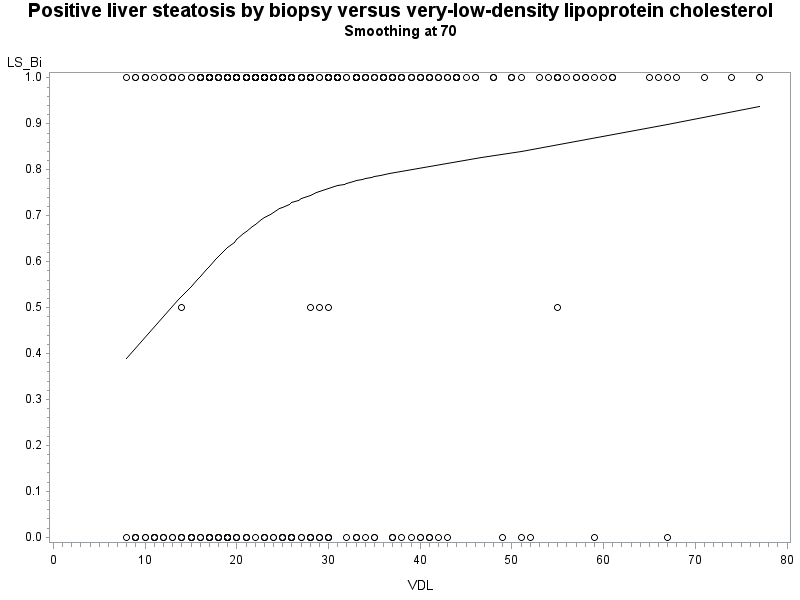
\includegraphics[width=0.5\textwidth]{/part1/lv}
\caption{Plot of LS\_Bi vs. VDL with a smooth curve. A curve is noted in the graph.}
\label{lv}
\end{figure}
\end{minipage} \hfill

The piecewise regression plot is provided below with two different lines used in the model (Figure \ref{pw}). There is one slope from VDL =5 to VDL = 25, and a different slope for VDL > 25.\\
\begin{minipage}{\textwidth}		
\begin{figure}[H]
\centering
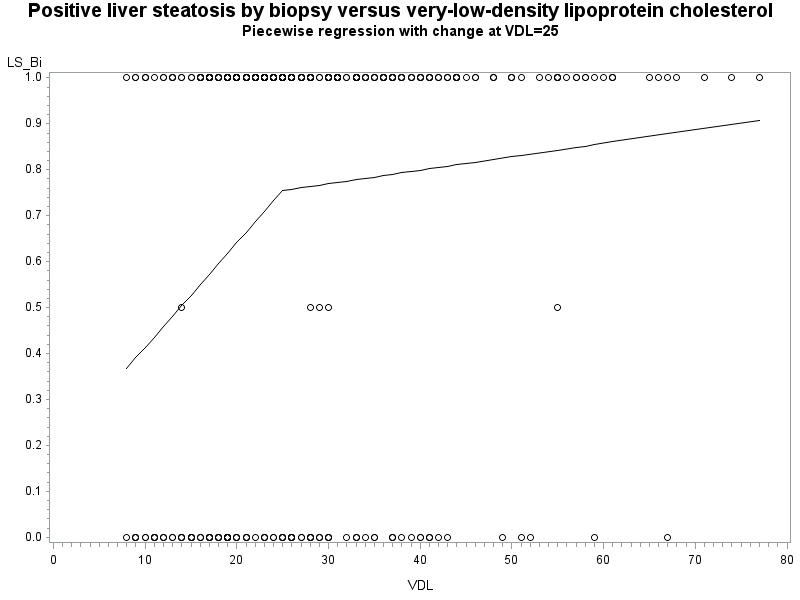
\includegraphics[width=0.5\textwidth]{/part1/pw}
\caption{Piecewise regression plot for modeling relationship between LS\_Bi and VDL}
\label{pw}
\end{figure}
\end{minipage} \hfill

The model used is:
\begin{align*}
LS\_Bi &= b_0 + b_1\cdot(VDL)+b_2X_3(VDL-25)\\
LS\_Bi &= b_0 + b_1\cdot (VDL)+b_2X_2(VDL-25)\\
&= b_0 -25b_2X_2 + b_1(VDL) + b_2X_2 \cdot VDL \\
&= {b_0 + b_1X_1 	X_2 = 0 (X_1 \leq 25)} \\
&= {(b_0 -25\cdot b_2X_2) + (b_2 + b_1)\cdot (VDL)	X_2 = 0  (X_1 > 25)}
\end{align*}

The test shows that the lines are different.
The hypotheses are:
\begin{align*}
H_0&: b_1=b_3=0\\
H_a&: \text{$b_1$ or $b_3$ are not zero}
\end{align*}

\begin{minipage}{\textwidth}
%\begin{table}
\centering
\captionof{table}{\small Test sameline Results for Dependent Variable LS\_Bi}
\begin{tabular}{c | c | c | c | c}
\hline
Source&	DF	&Mean square	&F Value	& $Pr>F$ \\
\hline
Numerator&	2&	2.77694	&14.41	& $<.0001$\\
\hline
Denominator	&390	&0.19272	 	 & & \\
\hline
\end{tabular}
%\end{table}
\end{minipage} \hfill

The F-statistic is 14.41. The numerator $df =2$, denominator $df =390$. The critical F-value is 3.087 with $\alpha = 0.05$. The corresponding p-value is very small ($<0.0001$). There is sufficient evidence to reject the null hypothesis and conclude that the two lines are not the same for the piecewise regression. This is also consistent with the visual observation made from the piecewise regression plot shown above.

\subsection{2. Extra Sums of Squares}

To better investigate implications of the extra sums of squares and the effects of changing model variables, a variable named SUM was created. This variable was the summation of the predictors ALT (alanine aminotransferase) and AST (aspartate aminotransferase). One reason behind selecting these two specific variables to sum is that they display a degree of correlation.This makes sense as they are both measurements of enzyme activity, and are both aminotransferase enzymes at that. The units for the two are also the same. \\

In order to test the effects of the new variable SUM, linear regression was run on the model of all explanatory variables including SUM and the model of all explanatory variables except for SUM. Note that neither test included SUM's component variables ALT and AST as their addition would be redundant. To better illustrate the effects, the model sum of squares was calculated based on the ANOVA results of the two regression models. This value was then used to calculate the F-statistic to test the null hypothesis that the coefficient for SUM equaled zero. The alternative hypothesis was that it did not equal zero.

% insert fig /part1prob2&3/mod1 %

% insert fig /part1prob2&3/mod2 %

Let $X_1,...,X_n$ represent all explanatory variables excluding AST, ALT, and SUM.
\begin{align*}
SSM(SUM | X_1,...,X_n) &=SSE(R)-SSE(F)\\
SSM(SUM | X_1,...,X_n) &=SSE(X_1,...,X_n)-SSE(SUM,X_1,...,X_n)\\
SSM(SUM | X_1,...,X_n) &=31.85979-31.68680=\fbox{0.17299}
\end{align*}
$$F=\frac{SSM/(df_E(R)-df_E(F))}{SSE(F)/df_E(F)}=\frac{0.17299/(334-333)}{31.6868/333}=\fbox{1.81797}$$

% insert fig /part1prob2&3/test %

The "test" statement was added to the regression statement in SAS to confirm the result. The conclusion drawn from these test statistics was to accept the null hypothesis. Running these models indicated that the inclusion of the variable SUM as a predictor did not improve the model.

\subsection{3. Type I and II Sums of Squares}

The regression process was again run in SAS, this time with the SS1 and SS2 options included in order to obtain the type I and type II sums of squares, respectively. The model included all explanatory variables except for SUM. The order of the variables was the same as they were in the original dataset.\\

% insert fig /part1prob2&3/SStable %
For all predictors but LS\_US, the sums of squares for type I and type II did not equal each other. For LS\_US the reason for the two sums being equal was because they were the last calculated, therefore not giving any meaningful interpretation. The sum of the type I sum of squares was 33.47034. The sum of the type II sum of squares was 20.99982. The model sum of squares equaled that of the total summation of the type I sum of squares. This is because the type I sum of squares is calculated in a hierarchal method, each calculation an adjustment of error based on each additional predictor. Because the regression model used did not deviate from the original dataset in its variable order, the calculated sum of squares also followed the same order as type I was calculated, due to the model sum of squares being equal to the reduced model SSE minus the full model SSE.\\

\subsection{4. Multiple linear regression models with different combinations of explanatory variables}
A set of 16 models were run in SAS. The model DF (number of coefficents not including the intercept), the model statement, $R^2$, and adjusted $R^2$ are reported. The models are sorted in ascending order of $R^2$ adjusted.  The $R^2$ adjusted ranges from 0.0689 to 0.5163, which shows that the the selection of explanatory variables significantly changes the amount of variation in the response variable, LS\_Bi, that can be explained by the linear regression model. \\

\begin{minipage}{\textwidth}
\centering
\captionof{table}{\small List of Variables from the Liver Steatosis Dataset} \label{vars}
\scalebox{.73}{
	\begin{tabular}{ | c | l | c | l | c |}
	\hline
	$DF_M$ &	\hspace{2in} Model	& $R^2$	& $R^2_{Adj}$ \\
	\hline
	6	& LS\_Bi=Age Sex Height Weight BMI SUM;	&0.0848 &	0.0689\\ \hline
	5	& LS\_Bi=Age Sex Height Weight SUM;	&0.0829	&0.0697\\\hline
	16	& LS\_Bi=Age Sex Height Weight BMI Obes DM Met HTN HPL TG CHOL HDL LDL VDL SUM;	&0.1519	&0.1115\\ \hline
	17	& LS\_Bi=Age Sex Height Weight BMI Obes DM Met HTN HPL TG CHOL HDL LDL VDL AST ALT SUM;	&0.1654	&0.123\\\hline
	6	& LS\_Bi=Age Sex Height Weight SUM LS\_US;	&0.3121	&0.302\\\hline
	18	& LS\_Bi=Age Sex Height Weight BMI Obes DM Met HTN HPL TG CHOL HDL LDL VDL NAS LS\_US SUM;	&0.5158	&0.4897\\\hline
	14	& LS\_Bi=Age Sex Height Weight BMI Obes DM Met HTN HPL NAS Fibrosis LS\_US SUM;	&0.5245	&0.5048\\\hline
	14	& LS\_Bi=Age Sex Height Weight BMI Obes DM Met HTN HPL NAS Fibrosis LS\_US SUM;	&0.5245	&0.5048\\\hline
	16	& LS\_Bi=BMI Obes DM Met HTN HPL TG CHOL HDL LDL VDL AST ALT NAS Fibrosis LS\_US SUM;&	0.5308	&0.5085\\\hline
	15	& LS\_Bi=BMI Obes DM Met HTN HPL TG CHOL HDL LDL VDL NAS Fibrosis LS\_US SUM;	&0.5296	&0.5087\\\hline
	15  & LS\_Bi=BMI Obes DM Met HTN HPL TG CHOL HDL LDL VDL NAS Fibrosis LS\_US SUM;	&0.5296&	0.5087\\\hline
	16	& LS\_Bi=Age Sex Height Weight BMI Obes DM Met HTN HPL TG CHOL NAS Fibrosis LS\_US SUM;&	0.5349&	0.5128\\\hline
	18	& LS\_Bi=Age Sex Height Weight BMI Obes DM Met HTN HPL TG HDL LDL VDL NAS Fibrosis LS\_US SUM;&	0.539&	0.5142\\\hline
	19 & LS\_Bi=Age Sex Height Weight BMI Obes DM Met HTN HPL TG CHOL HDL LDL VDL NAS Fibrosis LS\_US SUM;	&0.5406	&0.5143\\\hline
	17	& LS\_Bi=Age Sex Height Obes DM Met HTN HPL TG CHOL HDL LDL VDL NAS Fibrosis LS\_US SUM;&	0.5383	&0.5149\\\hline
	16	& LS\_Bi=Age Sex Height DM Met HTN HPL TG CHOL HDL LDL VDL NAS Fibrosis LS\_US SUM;	&0.5383	&0.5163 \\
	\hline
	\end{tabular}
}
\end{minipage} \hfill
%----------------------------------------------------------------------------------------
%	PART II
%----------------------------------------------------------------------------------------
\section{Part II}
\subsection{0. Overview}
In Part II, we use techniques taught in class to diagnose any issues with the model, remedy these issues and select the best model. The proposed objective is to develop a model that uses non-invasive predictors to predict liver steatosis. NAS and Fibrosis are obtained from liver biopsy, so they were dropped from further analysis. The following model selection and analysis are based on the remaining 19 variables.

\subsection{1. Scatterplot and correlation matrix}
Figure \ref{corr} shows the correlation matrix of the 19 variables in consideration. The response variable LS\_Bi is the last row and column on the correlation matrix. We also highlighted Pearson correlation equal or higher than 0.5 in red. Similarly the scatterplot matrix is $19 \times 19$ and it is shown in Figure \ref{scatter}. \\
\begin{minipage}{\textwidth}		
\begin{figure}[H]
\centering
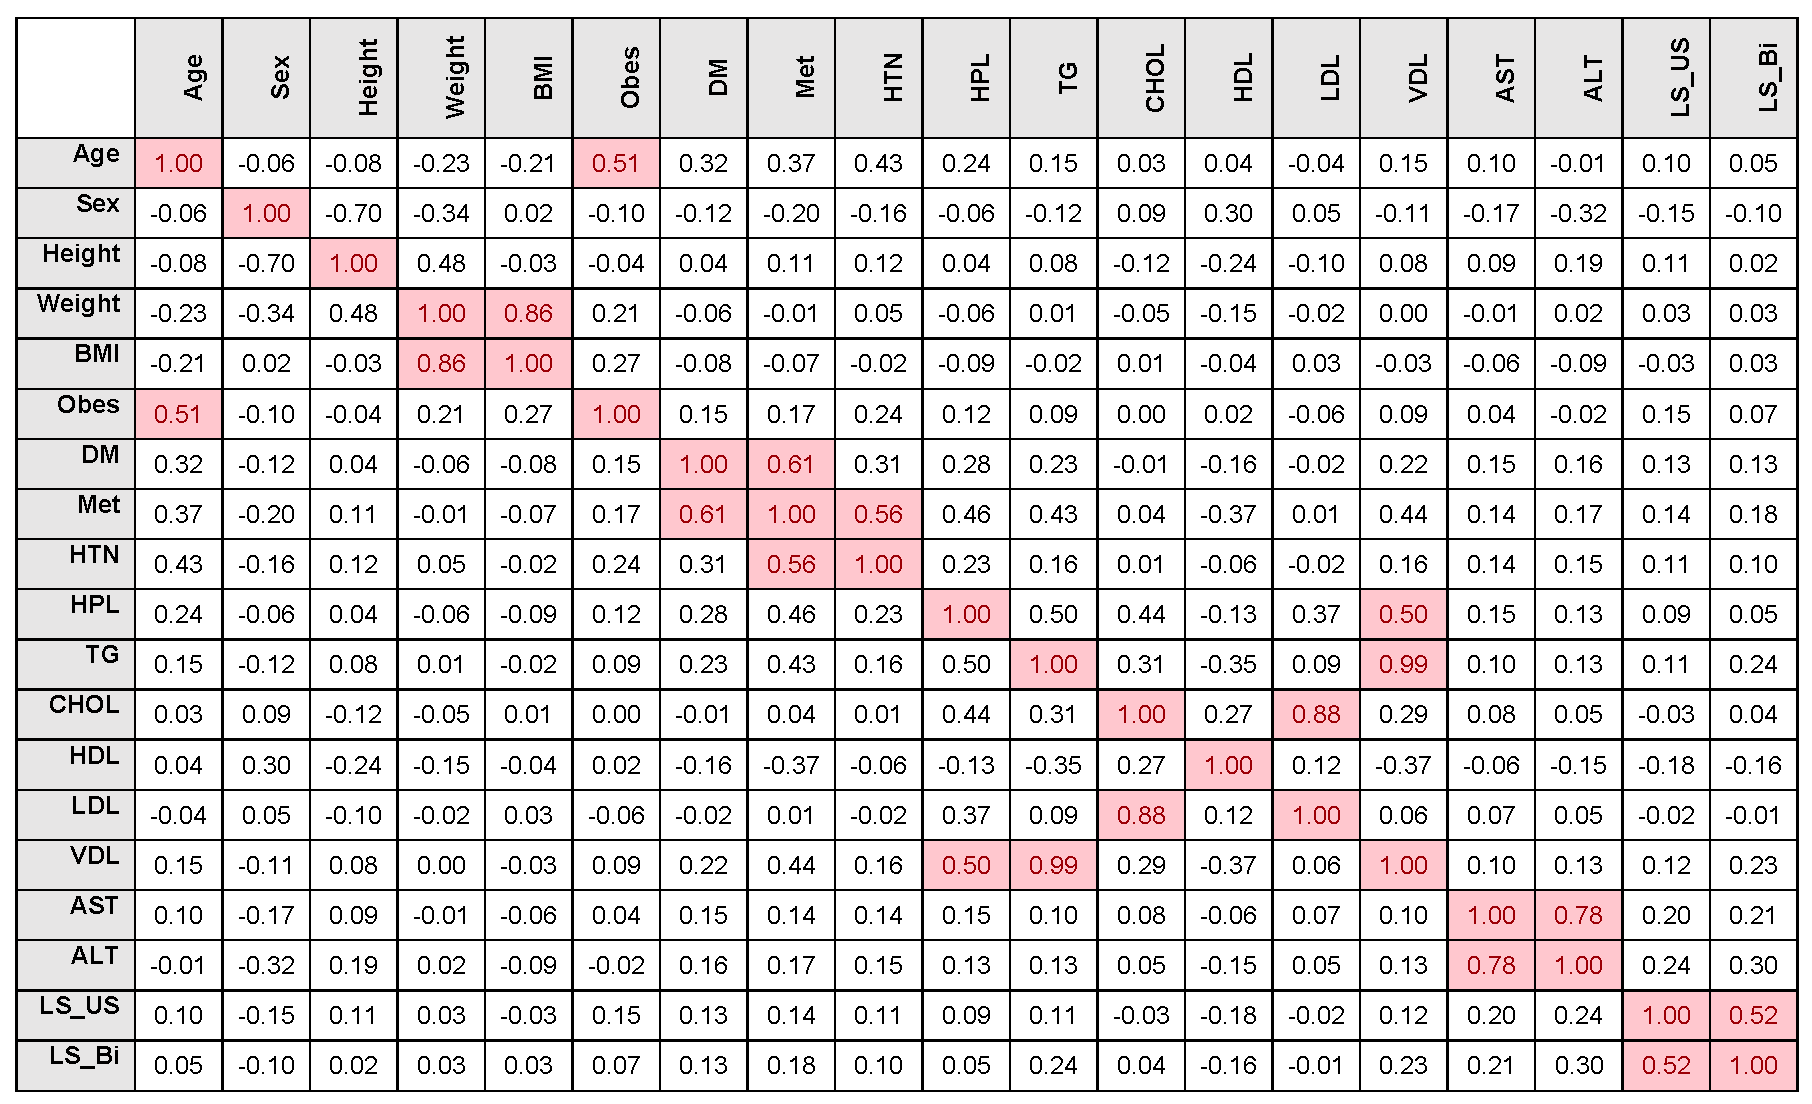
\includegraphics[width=0.7\textwidth]{/p1/corr_new2}
\caption{Correlation Matrix of Full Model Variables}
\label{corr}
\end{figure}
\end{minipage}

\begin{minipage}{\textwidth}		
\begin{figure}[H]
\centering
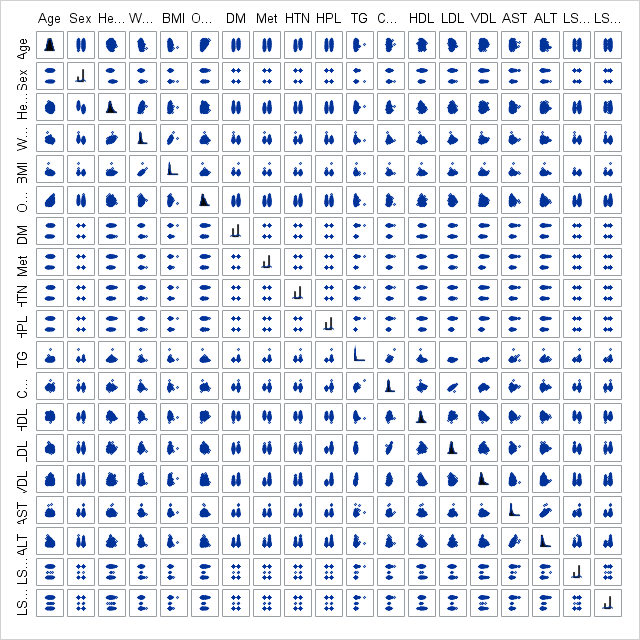
\includegraphics[width=0.8\textwidth]{/p1/SGScatter1}
\caption{Scatter Plots of All Variables}
\label{scatter}
\end{figure}
\end{minipage} \hfill

As is shown in the preceding plots, most variables are weakly correlated except for the follow pairs:
\begin{itemize}
	\item BMI is highly correlated to Weight with Pearson correlation at 0.86. 
	\item Met and DM are correlated, with Pearson correlation at 0.61.
	\item HTN and Met are moderately correlated with Pearson correlation at 0.56.
	\item VDL and TG are almost perfectly correlated with Pearson correlation at 0.99.
	\item LDL and CHOL are strongly correlated with Pearson correlation at 0.88.
	\item ALT and AST are correlated with Pearson correlation at 0.78.
	\item Fibrosis and NAS are correlated with Pearson correlation at 0.64.
	\item LS\_Bi and NAS are correlated with Pearson correlation at 0.63.
\end{itemize}

Correlation in explanatory variables will introduce multicolinearity to the model, and correlation on these pairs will be cloasely examined in the model selection. 

Additionally, it can also be noted that only LS\_US which is ultrasonic imagining of the liver is moderately correlated to the response variable. The $R^2$ is not expected to be high for the linear regression model.\\

For clarity, we recreated scatter plots pairs of variables with moderate or strong correlations, as are shown in Figure \ref{scatter2}. 

\begin {figure}
	\begin{tabular}{c c c c}
		\begin{minipage}{.23\textwidth}
		\centering		
		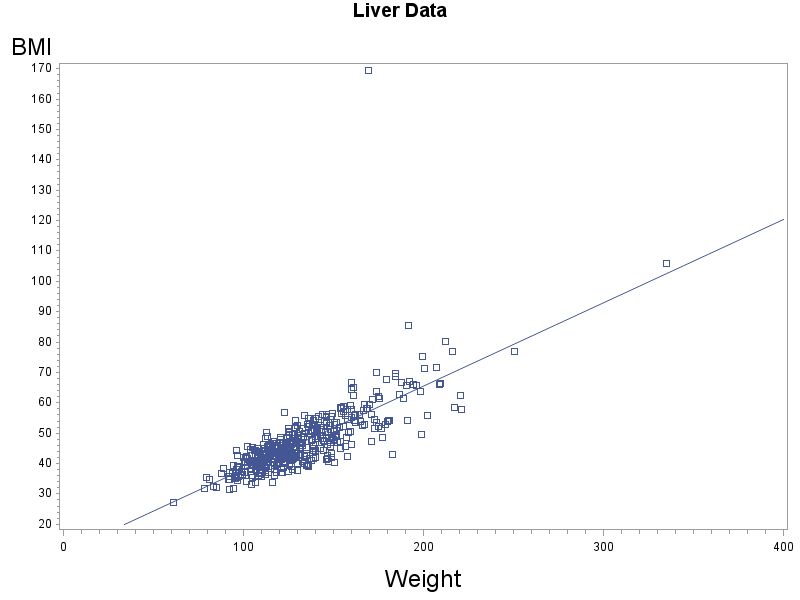
\includegraphics[width=0.99\textwidth]{/p1/bw}
		\end{minipage}
		&
		\begin{minipage}{.23\textwidth}
		\centering
		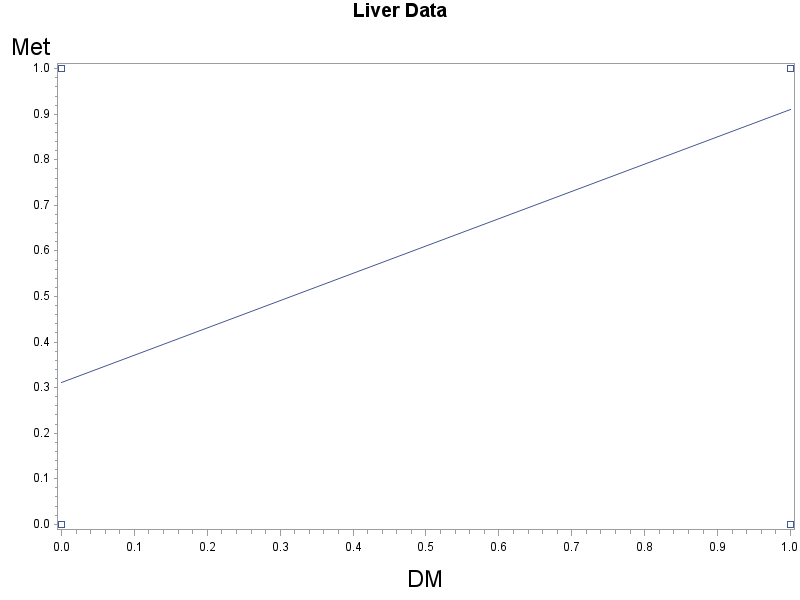
\includegraphics[width=0.99\textwidth]{/p1/md}
		\end{minipage}
		&
		\begin{minipage}{.23\textwidth}
		\centering
		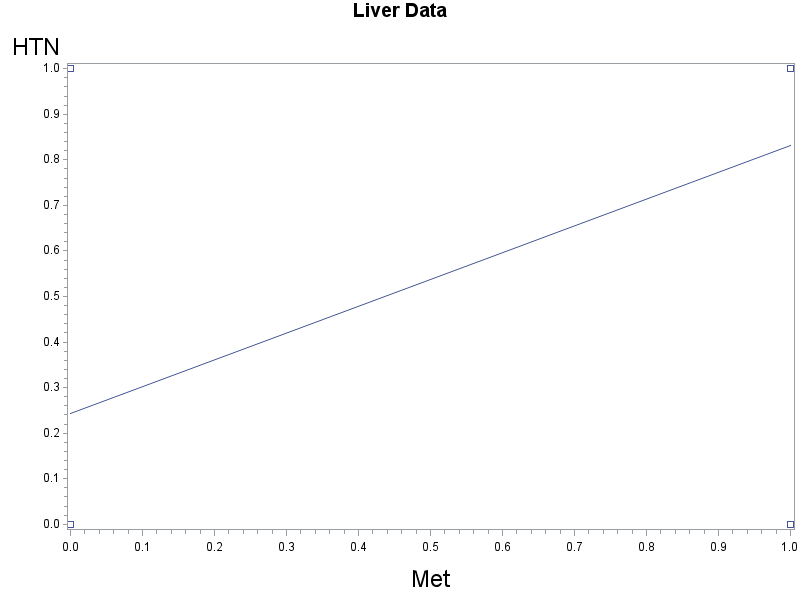
\includegraphics[width=0.99\textwidth]{/p1/hm}
		\end{minipage} 
		& 
		\begin{minipage}{.23\textwidth}
		\centering
		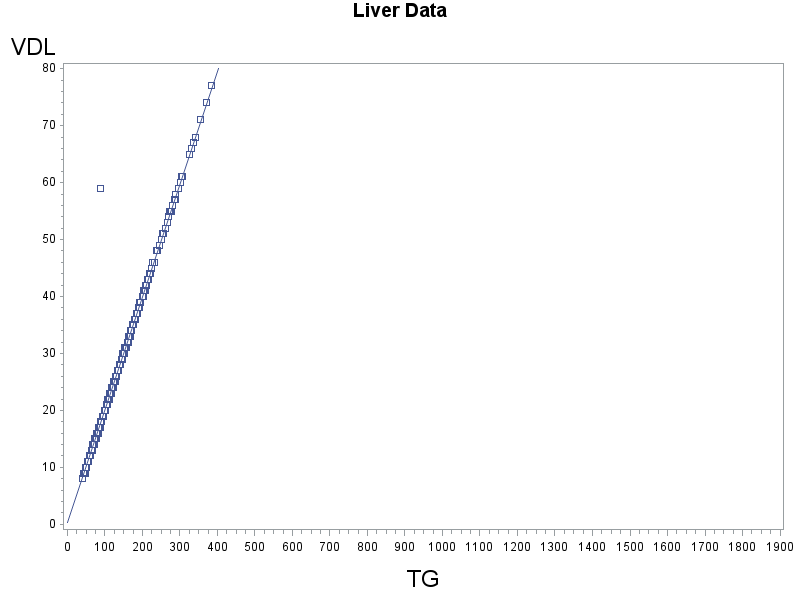
\includegraphics[width=0.99\textwidth]{/p1/vt}
		\end{minipage} 
		\\
		\begin{minipage}{.2\textwidth}
		\centering		
		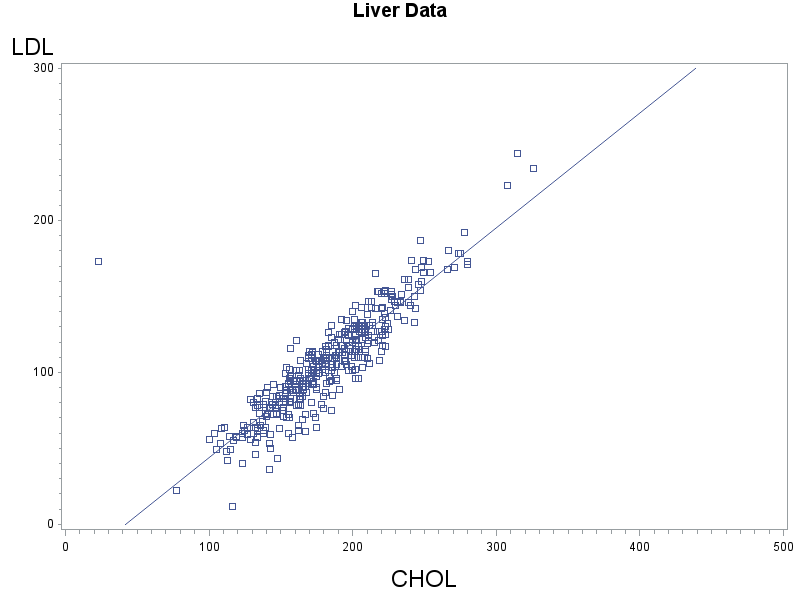
\includegraphics[width=0.99\textwidth]{/p1/lc}
		\end{minipage}
		&
		\begin{minipage}{.23\textwidth}
		\centering
		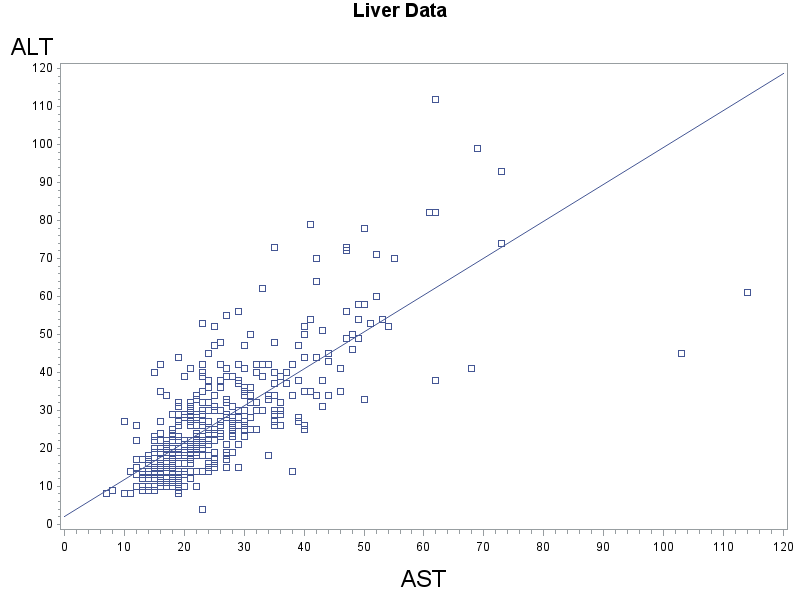
\includegraphics[width=0.99\textwidth]{/p1/aa}
		\end{minipage}
		&
		\begin{minipage}{.23\textwidth}
		\centering
		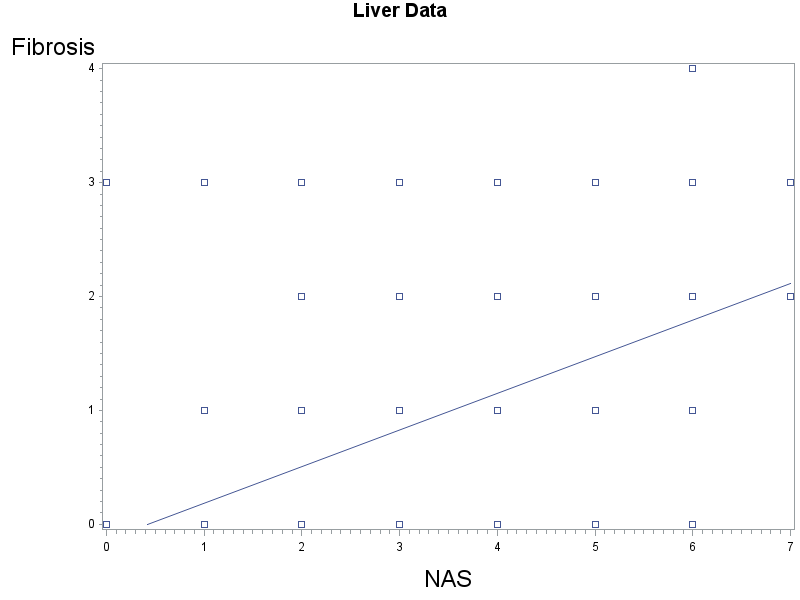
\includegraphics[width=0.99\textwidth]{/p1/fn}
		\end{minipage} 
		& 
		\begin{minipage}{.23\textwidth}
		\centering
		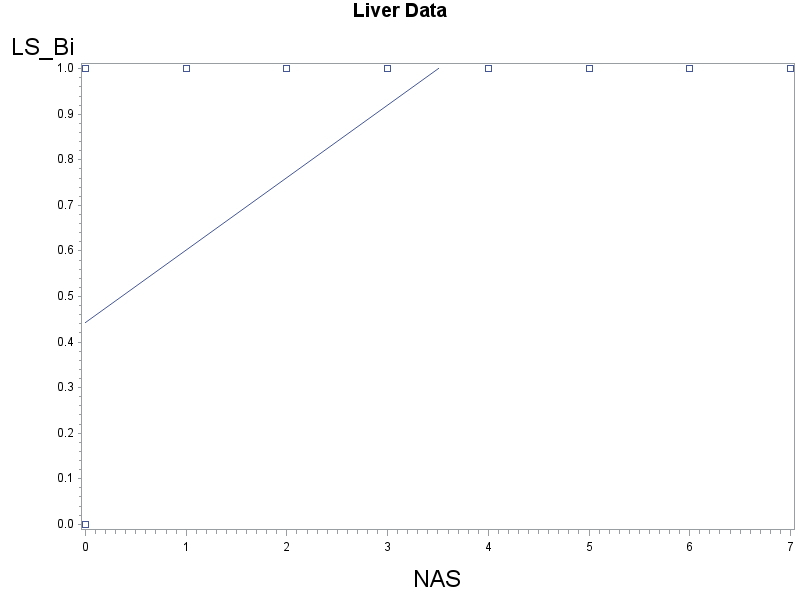
\includegraphics[width=0.99\textwidth]{/p1/ln}
		\end{minipage} 
	\end{tabular} \hfill
	\caption {Scatter Plots of Correlated Variables} \label{scatter2} 
\end{figure}


\subsection{2. Transformations}
We use the scatter plots and residual plots to check for possible transformation needed for our variables. Scatter plots are shown in Figure \ref{scatter} and Table \ref{scatter2} and the residual plots are shown in Figure \ref{resid}. \\

\begin{figure}
	\begin{tabular}{c c c}
	\begin{minipage}{.33\textwidth}
	\centering
	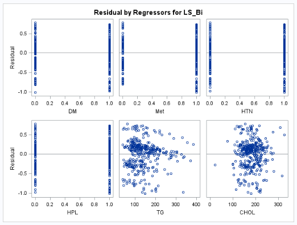
\includegraphics[width=0.99\textwidth]{/p2/re1b}
	\end{minipage}
	&
	\begin{minipage}{.33\textwidth}
	\centering
	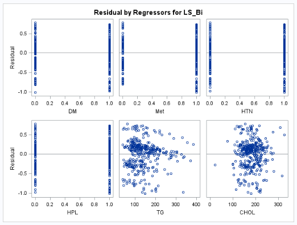
\includegraphics[width=0.99\textwidth]{/p2/re1b}
	\end{minipage}
	&
	\begin{minipage}{.33\textwidth}
	\centering
	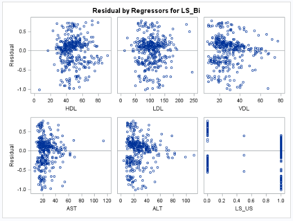
\includegraphics[width=0.99\textwidth]{/p2/re1c}
	\end{minipage}
	\end{tabular}
\caption {Scatter Plots of Correlated Variables} \label{resid} 
\end{figure}


As is shown, there is no nonlinear relationships between the residuals and the explanatory variables that can need to be corrected using transformation. It is apparent that the residuals are not constant as a function of the explanatory variables as evident in Figure 5. This necessiates transformation of the response variable, LS\_Bi. A Box-Cox procedure is applied and the best power tranformation returned from the SAS analysis is $\lambda = 0.5$, shown in Figure \ref{boxcox}. \\

\begin{minipage}{\textwidth}		
\begin{figure}[H]
\centering
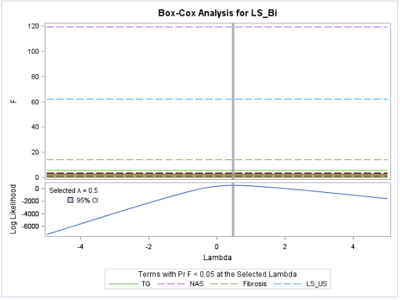
\includegraphics[width=0.5\textwidth]{/p2/boxcox}
\caption{Box Cox Transformation of LS\_Bi}
\label{boxcox}
\end{figure}
\end{minipage} \hfill


We apply this power transformation of Y and test for quality of the model. Note that since the response variable LS\_Bi is categorical and takes only 0 or 1, we increase this value by 1 to avoid 0 denominator in box-cox Transformation. \\

To determine the model quality, we use two measures: $R^2$ improvement and misclassification rate. The two measures for full model before and after the transformation is shown in the Table \ref{compare1}. \\

Note we use 0.5 as the threshold for classifying the model predicted $\hat{LS\_Bi}$, i.e. if $\hat{LS\_Bi} > 0.5$, the observation is classified as "liver steatosis positive", and otherwise, negative. This classification if contradicting with the observed LS\_Bi value, the observation will be counted toward misclassification. Therefore misclassificaiton rate is the percentage of unmatched model classification with observed LS\_Bi classification over the total observations. Observation with any missing values are not counted.\\


\begin{minipage}{\textwidth}
%\begin{table}
\centering
\captionof{table}{\small $R^2$ and Misclassification Rate Before and After Y transformation} \label{compare1}
	\begin{tabular}{c | c | c}
	\hline
	& Before & After\\
	\hline
	$R^2$ & 0.3644 & 0.3706 \\
	\hline
	Misclassification Rate & 0.188 & 0.172\\
	\hline
	\end{tabular}
%\end{table}
\end{minipage} \hfill

The residual plots for the transformed response variable is shown in Figure \ref{residTrans}. The plots indicate the little improves were made to the non-constant variance issue.\\

\begin{figure}
\begin{tabular}{c c c}
\begin{minipage}{.33\textwidth}
\centering
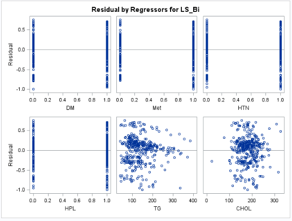
\includegraphics[width=0.99\textwidth]{/p2/re2b}
\end{minipage}
&
\begin{minipage}{.33\textwidth}
\centering
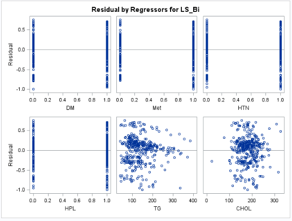
\includegraphics[width=0.99\textwidth]{/p2/re2b}
\end{minipage}
&
\begin{minipage}{.33\textwidth}
\centering
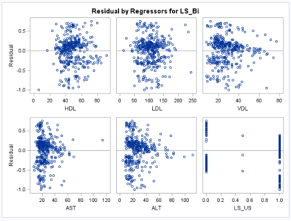
\includegraphics[width=0.99\textwidth]{/p2/re2c}
\end{minipage}
\end{tabular}
\caption {Scatter Plots of Correlated Variables} \label{residTrans} 
\end{figure}
Based on the little improvement and in favor of simpler model, we concluded no transformatoin is to be used for the response variable LS\_Bi.\\


%From the ANOVA table of the full model, we find the linear relationship to be significant with p-value of $<0.0001$. The parameter estimation show that TG, NAS, Fibrosis, and LS\_US are significant. From the correlation matrix, we noted strong correlations for certain variables and the parameter estimation confirms the effect of colinearity.\\

%Test Power Transformation, use Box-Cox transformation to find the best power transformation for the variables. \\

%\begin{minipage}{\textwidth}
%\begin{table}
%	\centering
%	\captionof{table}{Best $\lambda$ for Variables Box-Cox Transformation}
%	\begin{tabular}{|c | c |c | c |c | c |c | c |c | c |c |}
%	\hline
%	Age & Sex & Height & Weight & BMI & Obes & DM & MET & HTN & HPL & TG \\
%	\hline
%	1 & 4.5 & 0 & 1 & 0 & 0.5 & -- & -- & -- & -- & 1 \\
%	\hline
%	CHOL & HDL & LDL & VDL & AST & ALT & NAS & Fib & LS\_US & LS\_Bi & -- \\  
%	\hline
%	3 & 2 & 2.7 & 1 & 0 & 0.25 & -- & -- & -- & -- & -- \\
%	\hline
%	\end{tabular}
%\end{table}
%\end{minipage} \hfill


%\begin{minipage}{\textwidth}		
%\begin{figure}[H]
%\centering
%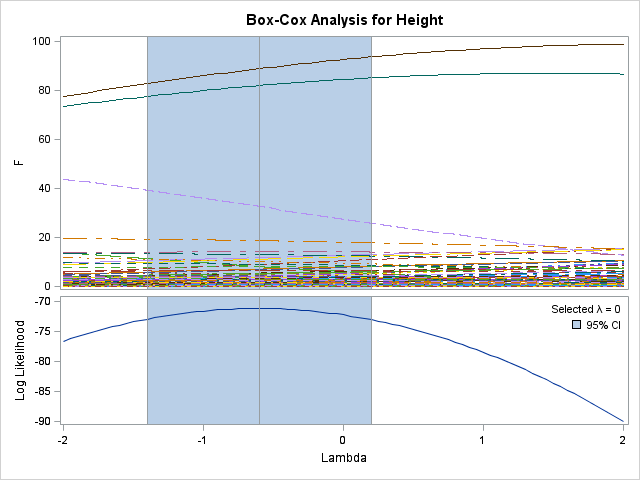
\includegraphics[width=0.551\textwidth]{/p2/index5/height}
%\end{figure}
%\end{minipage} \hfill
%
%\begin{tabular}{c c}
%\begin{minipage}{.5\textwidth}
%\centering		
%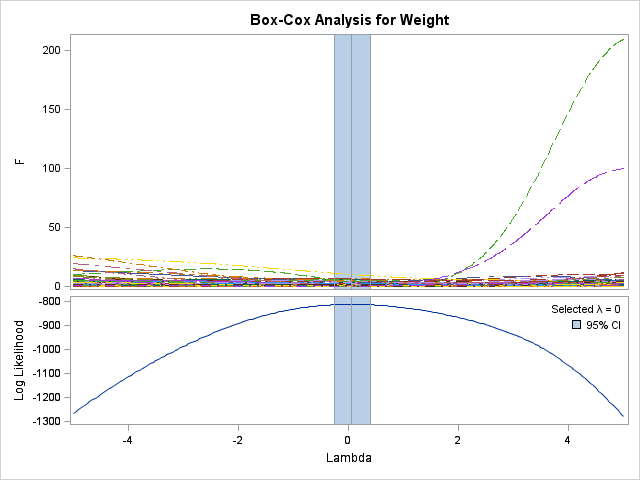
\includegraphics[width=0.99\textwidth]{/p2/index5/weight}
%\end{minipage}
%&
%\begin{minipage}{.5\textwidth}
%\centering
%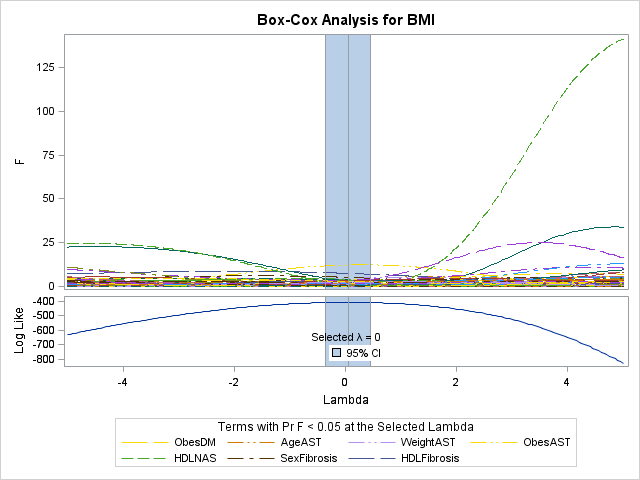
\includegraphics[width=0.99\textwidth]{/p2/index5/BMI}
%\end{minipage} 
%\\
%\begin{minipage}{.5\textwidth}
%\centering
%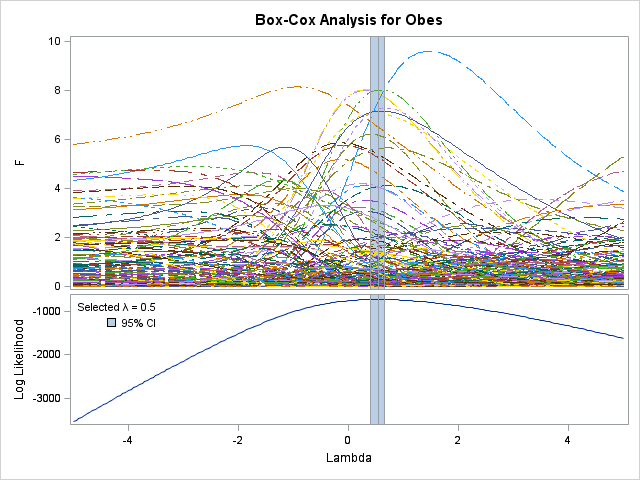
\includegraphics[width=0.99\textwidth]{/p2/index5/obes}
%\end{minipage} 
%& 
%\begin{minipage}{.5\textwidth}
%\centering
%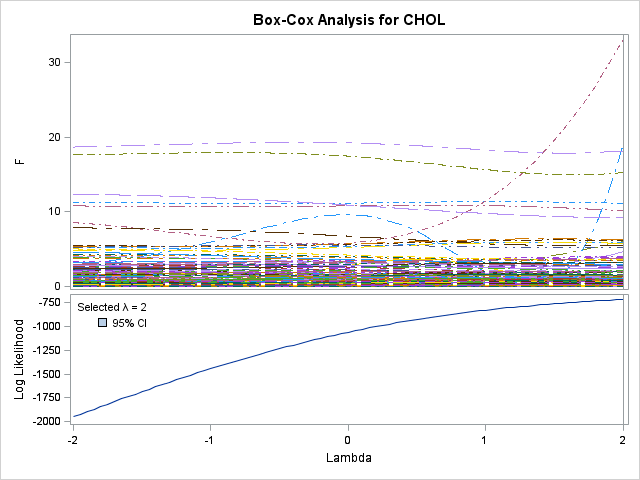
\includegraphics[width=0.99\textwidth]{/p2/index5/chol}
%\end{minipage} 
%\end{tabular} \hfill


\subsection{3. $C_p$ for Best Set of Variables}
The Cp criterion was used to select a regression model that explains the most variance in the response variable with the fewest number of explanatory variables. We conduct a model selection based on $C_p$, selecting the smallest model for $C_p \leq p$, which gives the best model with 9 variables: Weight, BMI, Met, HPL, TG, VDL, AST, ALT and LS\_US, as is shown in Table \ref{cp}.

\begin{minipage}{\textwidth}
	\captionof{table}{\small Model Selection Based on the $C_p$ Criteria} \label{cp}		
	\centering
	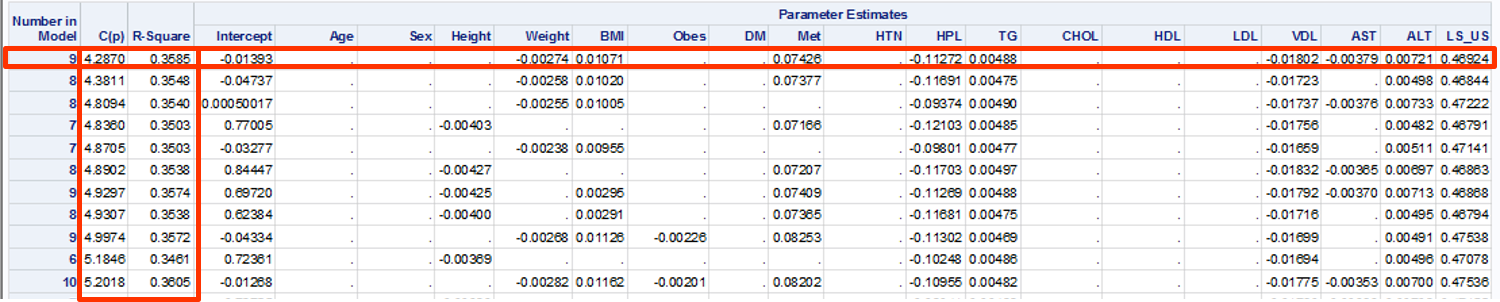
\includegraphics[width=0.99\textwidth]{/p3/cp}
\end{minipage} \hfill

We again measure the quality of this model with $R^2$ and misclassification rate. The values for the full model and this best model are listed in Table \ref{cpEval1}. \\

\begin{minipage}{\textwidth}
	\centering
	\captionof{table}{\small $R^2$ and Misclassification Rate for Full and Cp Models} \label{cpEval1}
	\begin{tabular}{c | c | c}
	\hline
	& Before & After\\
	\hline
	$R^2$ & 0.3644 & 0.3662 \\
	\hline
	Misclassification Rate & 0.188 & 0.190\\
	\hline
	\end{tabular}
\end{minipage} \hfill

From this comparison, $R^2$ again did not see significant improvement, and the misclassification rate is about the same. Yet with similar accuracy, this model is able to predict with only 9 variables down from 18. \\
Also note in this best model, we see that previously mentioned highly correlated pairs of variables are present. Significant multicollinearity among explanatory variables may lead to insignificant parameter estimation. It can be addressed by removing one of the highly correlated explanatory variables. This will be discussed further in the "best" model diagnostics section.\\

\subsection{4. Stepwise for Best Set of Variables}


The stepwise model selection in SAS returns a model with 6 variables: Height, Met, HPL, VDL, AST, and LS\_US, as is shown in Table \ref{sw}.\\
\begin{minipage}{\textwidth}		
\captionof{table}{\small Stepwise Model Selection} \label{sw}
\centering
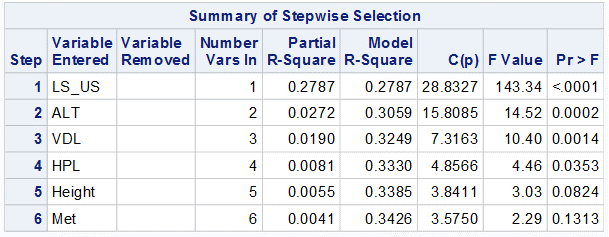
\includegraphics[width=0.7\textwidth]{/p4/sw}
\end{minipage} \hfill

We again measure the quality of this model with $R^2$ and misclassification rate. The values for the full model and this best model are listed in Table \ref{cpEval}. \\

\begin{minipage}{\textwidth}
\centering
\captionof{table}{\small $R^2$ and Misclassification Rate for Full and Cp Models} \label{cpEval}
\begin{tabular}{c | c | c}
\hline
& Before & After\\
\hline
$R^2$ & 0.3644 & 0.3260 \\
\hline
Misclassification Rate & 0.188 & 0.196\\
\hline
\end{tabular}
\end{minipage} \hfill

From this comparison, $R^2$ and the misclassification rate remain similar for the full model and selected best model. Not suprisingly, stepwise model remedied the multicolinearity issues the no longer have variables that are highly correlated.\\

\subsection{5. Assumptions Check}
%The assumptions of the linear regression model include linearity, constant variance, normality and independence. Due to the structure of the selected dataset, not all assumptions are expected to be met. In this section, we plot residuals, qqplots, histograms to examine these assumptions and interpret of the visual observations of these plots for implication on the assumptions as well as how they affect the model performance.\\
The model used for the rest of the questions has nine explanatory variables is provided below. The values of the regression coefficients are omitted for brevity.
\begin{align*}
LS\_Bi_{predicted} = &b_0 + b_1\cdot Weight + b2\cdot BMI + b3\cdot Metabolic\ Syndrome + b4\cdot Hyperlipidemia + \\ &b5 \cdot Plasma\ Triglycerides + b6\cdot Very\ Low\ Density\ Lipoprotein\ Cholesterol + \\ &b7 \cdot Aspartate\ Aminotransferase + b8 \cdot Alanine\ Aminotransferase + b9\cdot Ultrasound
\end{align*}

The model assumptions to evaluate are 1) linearity, 2) normality of residuals, 3) constant residuals as function of explanatory variables.\\

\textbf{Linearity:} LS\_Bi was plotted as a function of each of the explanatory variables used in the full model (Table \ref{cpScatter}). The variables Met, HPL, and LS\_US do not appear to have significant linearity issues with LS\_Bi, as evident by lack of curvature in the smooth lines for the plots shown in Figure 3. Curvature is observed in the plots for Weight, BMI, TG, VDL, AST and ALT. The curvature in Weight, BMI, TG, and AST appears to be due to outliers. Outliers and influential observations were examined in more detail in Part II, Problem 6. The curvature in ALT and VDL does not seem to be due to outliers. Power transformations were attempted for these variables but the not significantly improve the linearity of the relationship. Using piecewise regression for these two variables, as described in Part I, Problem I for  VDL, may be a possible remedy.\\
\begin{figure}[H]
\begin{tabular}{c c c}
\begin{minipage}{.32\textwidth}
\centering
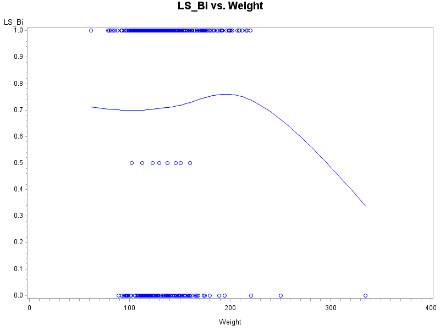
\includegraphics[width=0.99\textwidth]{/p5/5a}
\end{minipage}
&
\begin{minipage}{.32\textwidth}
\centering
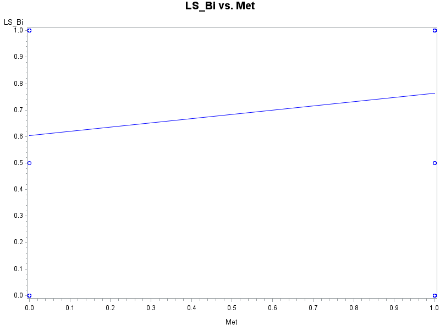
\includegraphics[width=0.99\textwidth]{/p5/5b}
\end{minipage}
&
\begin{minipage}{.3\textwidth}
\centering
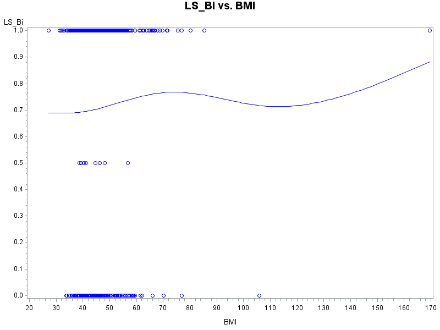
\includegraphics[width=0.99\textwidth]{/p5/5c}
\end{minipage}
\\
\begin{minipage}{.3\textwidth}
\centering
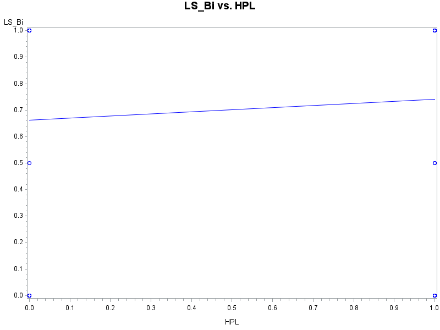
\includegraphics[width=0.99\textwidth]{/p5/5d}
\end{minipage}
&
\begin{minipage}{.3\textwidth}
\centering
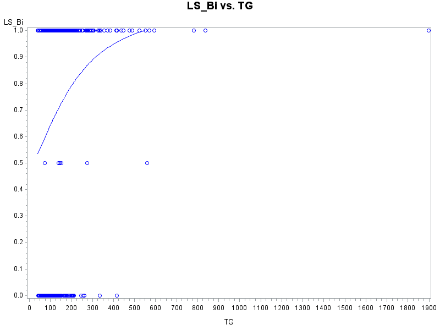
\includegraphics[width=0.99\textwidth]{/p5/5e}
\end{minipage}
&
\begin{minipage}{.3\textwidth}
\centering
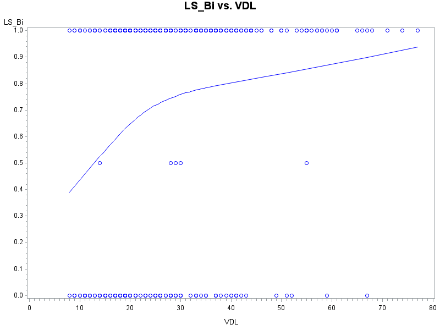
\includegraphics[width=0.99\textwidth]{/p5/5f}
\end{minipage}
\\
\begin{minipage}{.3\textwidth}
\centering
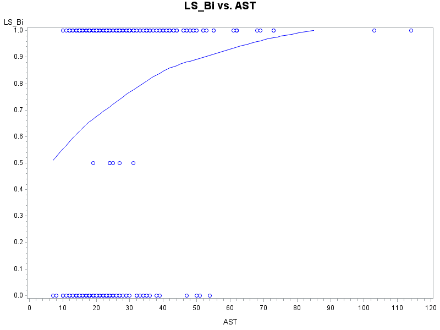
\includegraphics[width=0.99\textwidth]{/p5/5g}
\end{minipage}
&
\begin{minipage}{.3\textwidth}
\centering
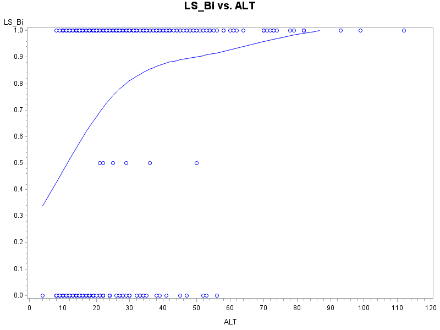
\includegraphics[width=0.99\textwidth]{/p5/5h}
\end{minipage}
&
\begin{minipage}{.3\textwidth}
\centering
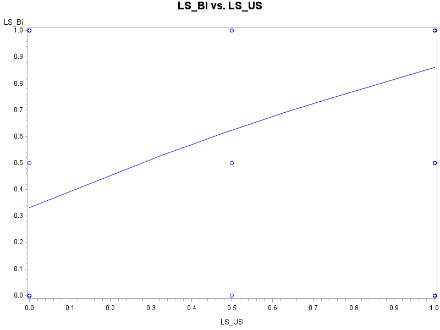
\includegraphics[width=0.99\textwidth]{/p5/5i}
\end{minipage}
\end{tabular}
\caption {Scatter plots of LS\_Bi vs the explanatory variables used in the model based on $C_p$ criterion} \label{cpScatter} 
\end{figure}

\textbf{Normality and homoscedasticity of residuals for full model:} Normality and homoscedasticity of residuals for full model: The QQ plot and histogram of the residuals for the “best” model are shown below in Figure \ref{norm}, along with the plot of the residuals vs. predicted values. Slight deviations from normality are seen in the QQ plot at the lower (-3 to -1) and higher (1 to 3) quantiles. The histogram appears fairly normal, but the distribution is skewed slightly to the right. Overall, the normality of the residuals seems sufficient for use in hypothesis testing that assume normality of the residuals. The residuals as a function of predicted value does not appear homoscedastic; the residuals tend to be positive at lower values of $LS\_Bi_{Predicted}$ and negative at higher values of $LS\_Bi_{Predicted}$. The lack of homoscedasticity of residuals in the model will cause issues in hypothesis testing.  \\

\begin{table}[H]
\centering
\caption {QQ plot and histogram of residuals for the model based on $C_p$ criterion} \label{norm} 
\begin{tabular}{c c c}
\begin{minipage}{.28\textwidth}
\centering
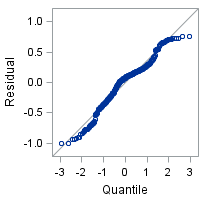
\includegraphics[width=0.99\textwidth]{/p5/n1}
\end{minipage}
&
\begin{minipage}{.28\textwidth}
\centering
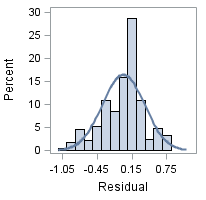
\includegraphics[width=0.99\textwidth]{/p5/n2}
\end{minipage}
&
\begin{minipage}{.28\textwidth}
\centering
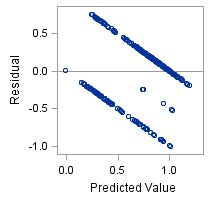
\includegraphics[width=0.99\textwidth]{/p5/n3}
\end{minipage}
\end{tabular}
\end{table}

\textbf{Constant residuals as function of explanatory variables:} This assumption is evaluated by plotting the model residuals as a function of each of the explantory variables. The partial residual plots are shown below in Figure \ref{residCp}.  The residuals for TG, VDL, AST, ALT, and LS\_US appear to have patterns or heteroscedastic. It does not appear that power transformations would be useful in significantly correcting the issues presented in the residuals for these variables. The residual plots for Weight, BMI, Met, HPL appear to be sufficiently homoscedastic. \\


\begin{table}[H]
	\centering
	\caption {Partial residual plots for the model based on $C_p$ criterion} \label{residCp} 
	\begin{tabular}{c}
	\begin{minipage}{.7\textwidth}
	\centering
	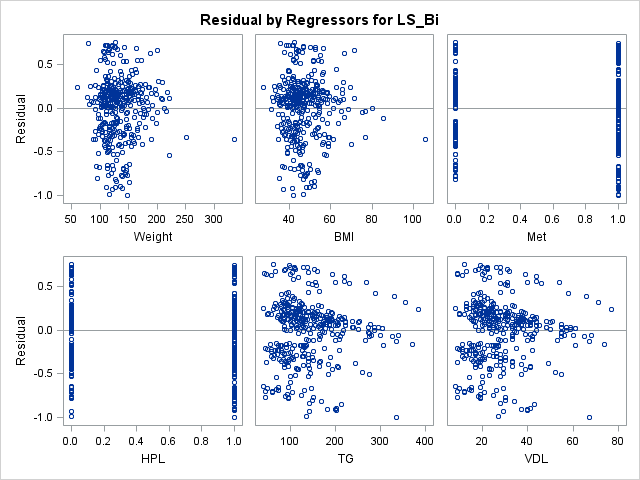
\includegraphics[width=0.99\textwidth]{/p5/r1}
	\end{minipage}
	\\
	\begin{minipage}{.7\textwidth}
	\centering
	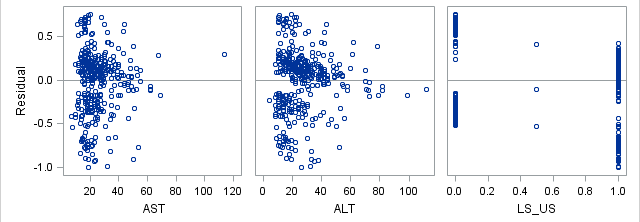
\includegraphics[width=0.99\textwidth]{/p5/r2}
	\end{minipage}
	\end{tabular}
\end{table}


%Independence: Again, referring to Table \ref{resid}, we can see that data poinsts are concentrated about a values and appear to be normally distributed. This is consistent with the sample where clinical and lab tests on the subjects are empirically normal. They are therefore not independent.

\subsection{6. Further model diagnostics and prediction of LS\_Bi (Outliers, influential observations, and multicollinearity)}

Outliers and influential observations were evaluated using studentized residuals, Cook’s D, and Hat Matrix. Visuals for these from the SAS outputs are provided in Table \ref{cook}. \\

The cutoff for the studentized residuals is calculated using $t_{n-p-1,(1-α/2n)} = t_{378-9-1, 1-0.05/(2\times378)} = t_{368, 0.99} \approx 3$. Values greater than three are considered outliers. None of the cases met this criterion so none are considered outliers based on studentized residuals.
\\

Cook’s D is used to detect influential observations. Cases with values greater than 4/n = 0.011 are considered overly influential based on this criterion. Cases 136,345, 287, 132, 121, 252, 217, 346, 249, 33, 175, 383 are above the Cook’s D threshold and are considered overly influential.\\

Finally, Hat Matrix diagonals were used to detect influential observations using the cutoff 2p/n = 0.0489. Cases 405,  379 ,94, 2, 273, 217, 368, 407, 347, 84, 230, 398, 346, 33, 383 are above the threshold and are considered overly influential. Removing these cases or giving them smaller weight in the regression model would improve the robustness of the model and may remedy some of the problems observed in the partial residual plots as discussed in problem 5. \\

Multicollinearity was evaluated using the variance inflation factor. A $VIF > 10$ indicates excessive multicollinearity among the explanatory variables. Based on the parameter estimate table provided below that includes the VIF, TG and VDL are highly correlated based the VIF of 36.5 and 36.8, respectively. The model would be improved by removing one of these variables. The high correlation of these variables was also noted in Part II, question 1. 

\begin{figure}[H]
\centering
\begin{tabular}{c c}
\begin{minipage}{.33\textwidth}
\centering
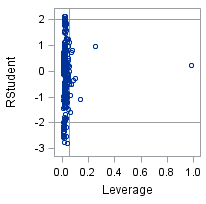
\includegraphics[width=0.99\textwidth]{/p6/a}
\end{minipage}
&
\begin{minipage}{.33\textwidth}
\centering
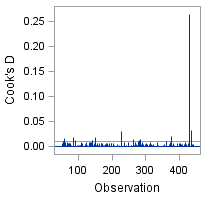
\includegraphics[width=0.99\textwidth]{/p6/b}
\end{minipage}
\end{tabular}
\caption{Studentized residual and Cook\' s D plots for the candidate model} \label{cook} 
\end{figure}


\begin{table}[H]
	\centering
	\caption{Parameter estimate table containing variance inflation factor} \label{pe} 
	\begin{tabular}{c}
	\begin{minipage}{.99\textwidth}
	\centering
	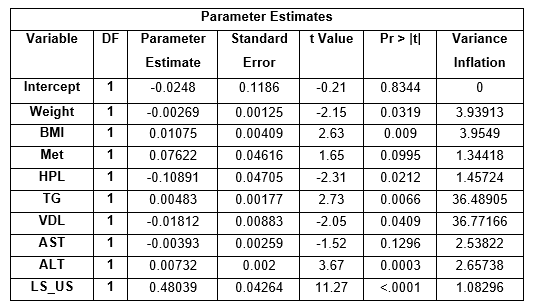
\includegraphics[width=0.65\textwidth]{/p6/pe}
	\end{minipage}
	\end{tabular}
\end{table}

The relationship between the predicted value of LS\_Bi and the observed value of LS\_Bi is shown below from the SAS output was well as in box-plots. The relationship is easier to visualize using the box plots due to the large number of data points at the discrete values of LS\_Bi. It is evident from the box plots that the predicted value of LS\_Bi tends to be higher for the cases where LS\_Bi is actually 1, indicating presence of liver steatosis.   However, there is a large spread in the data, and a significant amount of cases are predicted to have values of LS\_Bi that are less than 0.5 when the observed value of LS\_Bi is 1. 

\begin{minipage}{\textwidth}
	\begin{figure}[H]
	\centering
	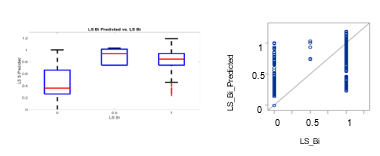
\includegraphics[width=0.6\textwidth]{/p6/pred}
	\caption{Plots relating the predicted value of LS\_Bi with the observed value of LS\_Bi}
	\end{figure}
\end{minipage}



\subsection{7. Equation of final model and inference on regression parameters and predicted values}
\textbf{Final Model:} The final regression model equation is provided below
\begin{align*}
LS\_Bi_{predicted} = - & 0.024 - 0.0027 \cdot Weight + 0.0108 \cdot BMI + 0.0762 \cdot (Metabolic\ Syndrome) - \\ &0.1089 \cdot (Hyperlipidemia) + 0.0048 \cdot (Plasma\ Triglycerides) -\\ &0.0181 \cdot (Very\ Low\ Density\ Lipoprotein\ Cholesterol) - \\ &0.0039 \cdot (Aspartate\ Aminotransferase) + 0.0073 \cdot (Alanine\ Aminotransferase) + \\ &0.4804 \cdot Ultrasound
\end{align*}

The table listing all of the 90\% confidence intervals for the mean value of the response variable (LS\_Bi) and the 90\% confidence interval for the individual observations are provided in Table \ref{predv}.\\

\begin{table}[H]
\centering
\caption{\small LS\_Bi predicted and 90\% prediction intervals of mean and individual observations for all cases} \label{predv} 
\begin{tabular}{c}
\begin{minipage}{\textwidth}
\centering
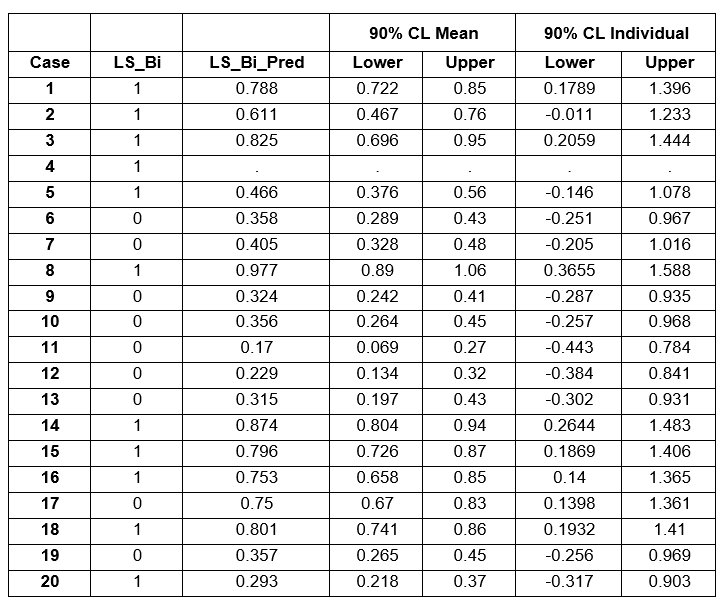
\includegraphics[width=0.65\textwidth]{/p7/top20}
\end{minipage}
\end{tabular}
\end{table}

The parameter estimate table with 90\% confidence intervals for the regression coeficients is provided in Table \ref{finalpe}:

\begin{table}[H]
\centering
\caption{\small Parameter estimate table containing 90\% confidence intervals for the regression coefficients} \label{finalpe} 
\begin{tabular}{c}
\begin{minipage}{\textwidth}
\centering
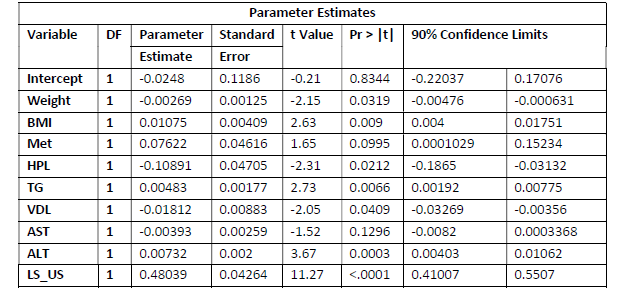
\includegraphics[width=0.8\textwidth]{/p7/fpe}
\end{minipage}
\end{tabular}
\end{table}

\section{Concluding Remarks}
The accuracy of the proposed model using a mix of clinical variables, blood test results, and liver ultrasound imaging to predict liver steatosis does not match that of liver biopsy. The proposed model may be useful in screening patients for biopsy. There is a large spread in the predicted values of LS\_Bi, and a significant amount of cases are predicted to have values of LS\_Bi that are less than 0.5 when the observed value of LS\_Bi is 1. It is not clear what the parameter estimates resulting from our analyses mean since they are being used to predict a categorical variable. This may limit the amount of scientific knowledge that can be derived from the model. The parameter estimates table shows that the ultrasound imaging, plasma triglycerides, alanine aminotransferase, and BMI are highly significant in explaining the variance in LS\_Bi. These variables should be explored in detail in further studies to understand if any causal relationship between them and liver steatosis exists. Further studies should perform the analysis with multiple logistic regression model which would provide more accurate parameter estimates. Finally, additional explanatory variables could be added to improve the predictive performance of the model.

\begin{thebibliography}{99}
	\bibitem{wu2011}
	Wu J, You J, Yerian L, Shiba A, Schauer PR, Sessler DI. Prevalence of liver steatosis and fibrosis and the diagnostic accuracy of ultrasound in bariatric surgery patients. Obesity surgery. 2011;22(2):240-7. 
	
	\bibitem{brunt2010}
	Brunt EM, Tiniakos DG. Histopathology of nonalcoholic fatty liver disease. World journal of gastroenterology. 2010;16(42):5286-96. 
	
	\bibitem{brunt2011}
	Brunt EM, Kleiner DE, Wilson LA, Belt P, Neuschwander-Tetri BA. The NAS and The Histopathologic Diagnosis in NAFLD: Distinct Clinicopathologic Meanings. Hepatology. 2011;53(3):810-20. 
	
\end{thebibliography}

%%%%%%%%%%%%%THE END%%%%%%%%%%%%%%%%%%%%%%%%
\end{document}